This Chapter summarises the structure of the information necessary to define
a PSHA input model to be used with the \glsdesc{acr:oqe}.

Input data for probabilistic based seismic hazard analysis (Classical, Event
based, Disaggregation, and Uniform Hazard Spectra) are organised into:

\begin{itemize}

	\item A general configuration file.

    \item A file describing the Seismic Source System, that is the set of
	initial source models and associated epistemic uncertainties needed to
	model the seismic activity in the region of interest.

    \item A file describing the Ground Motion System, that is the set of
	ground motion prediction equations, per tectonic region type, needed to
	model the ground motion shaking in the region of interest.

\end{itemize}

Figure~\ref{fig:psha_input} summarises the structure of a PSHA input model
for the \glsdesc{acr:oqe} and the relationships between the different files.

\begin{figure}[!ht]
\centering
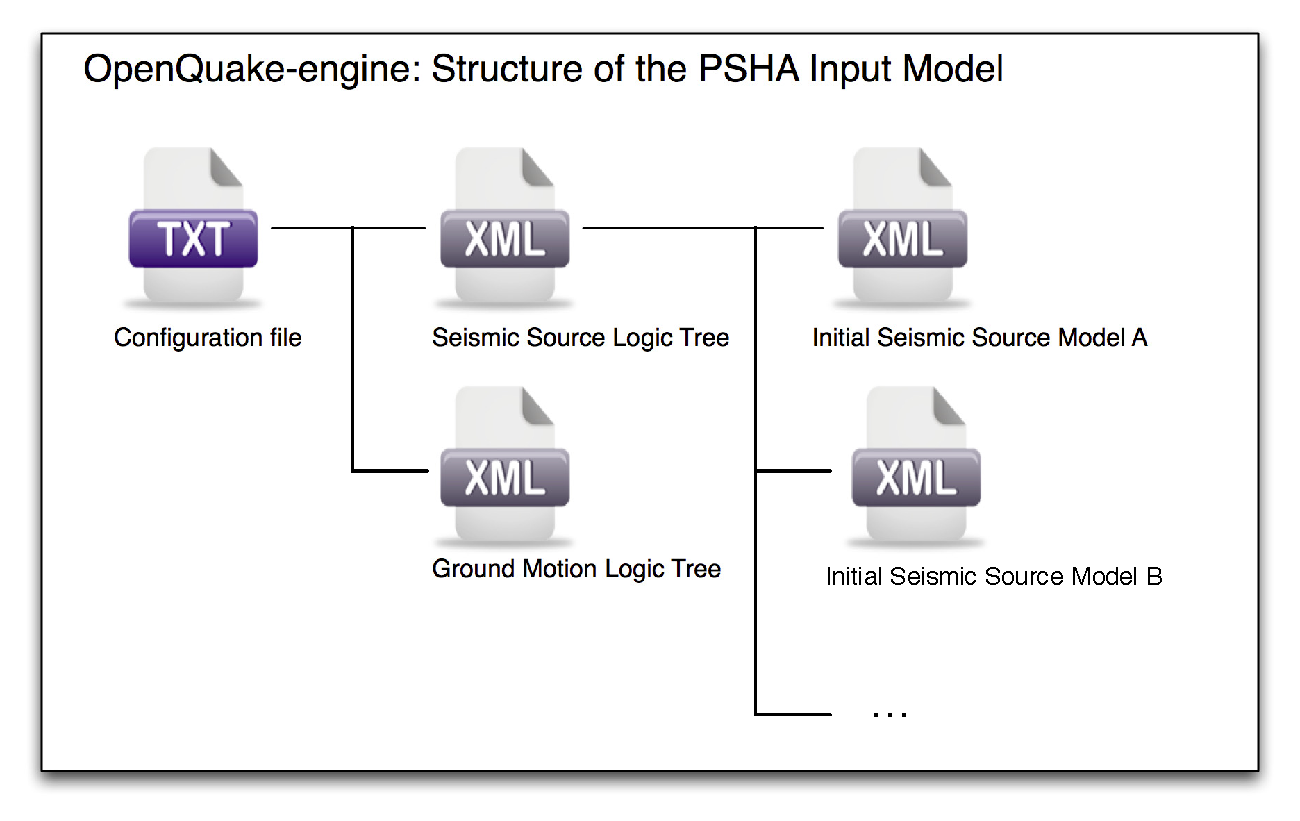
\includegraphics[width=14cm]{figures/hazard/psha_input_structure.pdf}
\caption{PSHA Input Model structure}
\label{fig:psha_input}
\end{figure}


\section{Defining Logic Trees}
The main components of a logic tree structure in the \glsdesc{acr:oqe} are the
following:

\begin{description}

    \item[branch]: the simplest component of a logic tree structure. A branch
	represent a possible interpretation of a value assignment for a specific type
	of uncertainty. It is fully described by the tuple (parameter or model,
	weight).

    \item[branching set]: it is a key component in the logic tree structure
	used by the \gls{acr:oqe}. It groups a set of branches i.e. alternative
	interpretations of a parameter or a model. Each branching set is defined by:

    \begin{itemize}

        \item An ID

        \item An uncertainty type (for a comprehensive list of the types of
		uncertainty currently supported see page~\pageref{list_epistemic_unc})

        \item One or more branches

    \end{itemize}

    This set of uncertainties can be applied to the whole initial  seismic
    source input model or just to a subset of seismic sources. The sum of the
    weights/probabilities assigned to the set  of branches always correspond
    to one.

\end{description}

Below we provide a simple schema illustrating the skeleton of xml file
containing the desciption of a logic tree:

\begin{minted}[firstline=1,firstnumber=1,fontsize=\footnotesize,frame=single,bgcolor=lightgray]{xml}
    <logicTreeBranchSet branchSetID=ID
                        uncertaintyType=TYPE>
        <logicTreeBranch>
            <uncertaintyModel>VALUE</uncertaintyModel>
            <uncertaintyWeight>WEIGHT</uncertaintyWeight>
        </logicTreeBranch>
    </logicTreeBranchSet>
\end{minted}

As it appears from this example, the structure of a logic tree is a set of
nested elements.

A schematic representation of the elemental components of a logic tree
structure is provided in Figure~\ref{glts}.
A branch set identifies a collection of
branches (i.e. individual branches)  whose weights sum to 1.

\begin{figure}[!ht]
\centering
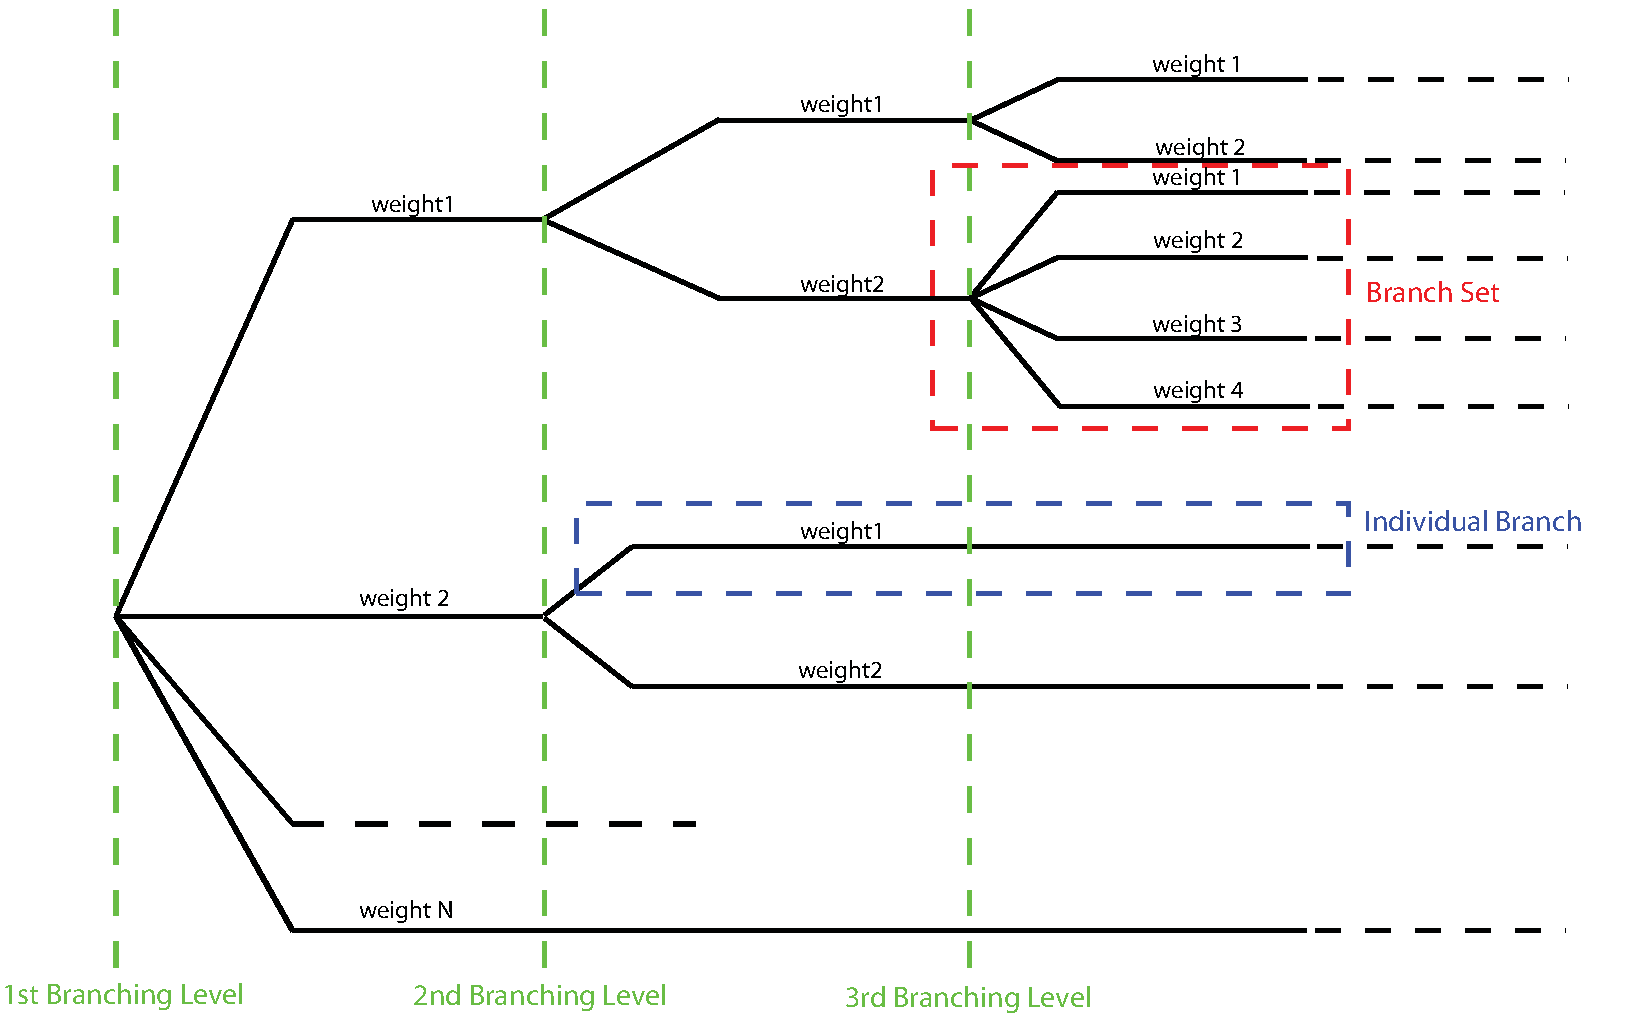
\includegraphics[width=13cm]{figures/hazard/GenericLogicTreeStructure.pdf}
\caption{Generic Logic Tree structure as described in terms of branch sets,
and individual branches.}
\label{glts}
\end{figure}

\subsection{Logic trees as described in the nrml schema}

In the NRML schema, a logic tree structure is defined through the
\Verb+logicTree+ element:

\begin{minted}[firstline=1,firstnumber=1,fontsize=\footnotesize,frame=single,bgcolor=lightgray]{xml}
<logicTree logicTreeID="ID">
...
</logicTree>
\end{minted}

A \Verb+logicTree+ contains as a sequence of \Verb+logicTreeBranchSet+ elements.

There are no restrictions on the number of branch set that can be defined.

Each \Verb+logicTreeBranchSet+
has two required attributes: \Verb+branchSetID+ and
\Verb+uncertaintyType+. The latter defines the type of epistemic uncertainty this branch set is describing.

\begin{minted}[firstline=1,firstnumber=1,fontsize=\footnotesize,frame=single,bgcolor=lightgray]{xml}
<logicTree logicTreeID="ID">
		<logicTreeBranchSet branchSetID="ID_1"
			uncertaintyType="UNCERTAINTY_TYPE">
			...
		</logicTreeBranchSet>
		<logicTreeBranchSet branchSetID="ID_2"
			uncertaintyType="UNCERTAINTY_TYPE">
			...
		</logicTreeBranchSet>
		...
		<logicTreeBranchSet branchSetID="ID_N"
			uncertaintyType="UNCERTAINTY_TYPE">
			...
		</logicTreeBranchSet>
...
</logicTree>
\end{minted}

Possible values for the \Verb+uncertaintyType+ attribute are:

\label{list_epistemic_unc}
\begin{itemize}

    \item \Verb+gmpeModel+: indicates epistemic uncertainties on ground
	motion prediction equations

	\item \Verb+sourceModel+: indicates epistemic uncertainties on source models

    \item \Verb+maxMagGRRelative+: indicates relative (i.e. increments)
	epistemic uncertainties to be added (or subtracted, depending on the sign
	of the increment) to the Gutenberg-Richter maximum magnitude value.

    \item \Verb+bGRRelative+: indicates relative epistemic uncertainties
	to be applied to the Gutenberg-Richter b value.

    \item \Verb+abGRAbsolute+: indicates absolute (i.e. values used to replace
	original values) epistemic uncertainties on the Gutenberg-Richter a and b
	values.

    \item \Verb+maxMagGRAbsolute+: indicates (absolute) epistemic
	uncertainties on the Gutenberg-Richter maximum magnitude.
	
	\item \Verb+incrementalMFDAbsolute+: indicates (absolute) epistemic uncertainties on the incremental magnitude frequency distribution (i.e. alternative rates and/or minimum magnitude) of a specific source (can only be applied to individual sources)
	
	\item \Verb+simpleFaultGeometryAbsolute+: indicates alternative representations of the simple fault geometry for an individual simple fault source
	
	\item \Verb+simpleFaultDipRelative+: indicates a relative increase or decrease in fault dip for one or more simple fault sources
	
	\item \Verb+simpleFaultDipAbsolute+: indicates alternative values of fault dip for one or more simple fault sources
	
	\item \Verb+complexFaultGeometryAbsolute+: indicates alternative representations of complex fault geometry for an individual complex fault source

	\item \Verb+characteristicFaultGeometryAbsolute+: indicates alternative representations of the characteristic fault geometry for an individual characteristic fault source

\end{itemize}

A \Verb+branchSet+ is defined as a sequence of \Verb+logicTreeBranch+
elements, each specified by an \Verb+uncertaintyModel+ element (a string
identifying an uncertainty model; the content of the string varies with the \texttt{uncertaintyType} attribute value of the branchSet element) and the \texttt{uncertaintyWeight} element (specifying the probability/weight associated to the uncertaintyModel):

\begin{minted}[firstline=1,firstnumber=1,fontsize=\footnotesize,frame=single,bgcolor=lightgray]{xml}
< logicTree  logicTreeID="ID">
...

		< logicTreeBranchSet  branchSetID="ID_#"
				uncertaintyType="UNCERTAINTY_TYPE">
			< logicTreeBranch  branchID="ID_1">
				<uncertaintyModel>
				    UNCERTAINTY_MODEL
				</uncertaintyModel>
				<uncertaintyWeight>
				    UNCERTAINTY_WEIGHT
				</uncertaintyWeight>
			</ logicTreeBranch >
			...
			< logicTreeBranch  branchID="ID_N">
				<uncertaintyModel>
				    UNCERTAINTY_MODEL
				</uncertaintyModel>
				<uncertaintyWeight>
				    UNCERTAINTY_WEIGHT
				</uncertaintyWeight>
			</logicTreeBranch>
		</logicTreeBranchSet>
...
</logicTree >
\end{minted}

Depending on the \Verb+uncertaintyType+ the content of the
\Verb+<uncertaintyModel>+ element changes:

\begin{itemize}

    \item if \Verb+uncertaintyType="gmpeModel"+, the uncertainty model
	contains the name of a ground motion prediction equation (a list of
	available GMPEs can be obtained using \texttt{oq info -g} or 
	\texttt{oq info --gsims} and these are also documented at:
	\href{http://docs.openquake.org/oq-engine/2.8/openquake.hazardlib.gsim.html}{http://docs.openquake.org/oq-engine/2.8/openquake.hazardlib.gsim.html}):

    \begin{minted}[firstline=1,firstnumber=1,fontsize=\footnotesize,frame=single,bgcolor=lightgray]{xml}
<uncertaintyModel>GMPE_NAME</uncertaintyModel>
	\end{minted}

    \item if \Verb+uncertaintyType="sourceModel"+, the uncertainty model
	contains the paths to a source model file, e.g.:

    \begin{minted}[firstline=1,firstnumber=1,fontsize=\footnotesize,frame=single,bgcolor=lightgray]{xml}
<uncertaintyModel>SOURCE_MODEL_FILE_PATH</uncertaintyModel>
	\end{minted}

    \item if \Verb+uncertaintyType="maxMagGRRelative"+, the uncertainty model
	contains the increment to be added (or subtracted, depending on the sign)
	to the Gutenberg-Richter maximum magnitude:

    \begin{minted}[firstline=1,firstnumber=1,fontsize=\footnotesize,frame=single,bgcolor=lightgray]{xml}
<uncertaintyModel>MAX_MAGNITUDE_INCREMENT</uncertaintyModel>
	\end{minted}

    \item if \Verb+uncertaintyType="bGRRelative"+, the uncertainty model
	contains the increment to be added (or subtracted, depending on the sign)
	to the Gutenberg-Richter b value:

    \begin{minted}[firstline=1,firstnumber=1,fontsize=\footnotesize,frame=single,bgcolor=lightgray]{xml}
<uncertaintyModel>B_VALUE_INCREMENT</uncertaintyModel>
	\end{minted}

    \item if \Verb+uncertaintyType="abGRAbsolute"+, the uncertainty model
	must contain one a and b pair:

    \begin{minted}[firstline=1,firstnumber=1,fontsize=\footnotesize,frame=single,bgcolor=lightgray]{xml}
<uncertaintyModel>A_VALUE B_VALUE</uncertaintyModel>
	\end{minted}

    \item if \Verb+uncertaintyType="maxMagGRAbsolute"+, the uncertainty
	model must contain one Gutenberg-Richter maximum magnitude value:

    \begin{minted}[firstline=1,firstnumber=1,fontsize=\footnotesize,frame=single,bgcolor=lightgray]{xml}
<uncertaintyModel>MAX_MAGNITUDE</uncertaintyModel>
	\end{minted}
	
	\item if \Verb+uncertaintyType="incrementalMFDAbsolute"+, the uncertainty model must contain an instance of the incremental MFD node:
	
    \begin{minted}[firstline=1,firstnumber=1,fontsize=\footnotesize,frame=single,bgcolor=lightgray]{xml}
<uncertaintyModel>
    <incrementalMFD
        minMag="MIN MAGNITUDE"
        binWidth="BIN WIDTH">
        <occurRates>RATE_1 RATE_2 ... RATE_N</occurRates>
    </incrementalMFD>
</uncertaintyModel>
    \end{minted}

    \item if \Verb+uncertaintyType="simpleFaultGeometryAbsolute"+ then the uncertainty model must contain a \emph{valid} instance of the \verb+simpleFaultGeometry+ node as described in section \ref{desc_simple_fault}

    \item if \Verb+uncertaintyType="simpleFaultDipRelative"+ then the uncertainty model must specify the number of degrees to increase (positive) or decrease (negative) the fault dip. Note that if this increase results in an adjusted fault dip greater than $90^{\circ}$ or less than $0^{\circ}$ an error will occur.
     
    \begin{minted}[firstline=1,firstnumber=1,fontsize=\footnotesize,frame=single,bgcolor=lightgray]{xml}
<uncertaintyModel>DIP_INCREMENT</uncertaintyModel>
	\end{minted}

	\item if \Verb+uncertaintyType="simpleFaultDipAbsolute"+ then the uncertainty model must specify the dip angle (in degrees)

    \begin{minted}[firstline=1,firstnumber=1,fontsize=\footnotesize,frame=single,bgcolor=lightgray]{xml}
<uncertaintyModel>DIP</uncertaintyModel>
	\end{minted}

    \item if \Verb+uncertaintyType="complexFaultGeometryAbsolute"+ then the uncertainty model must contain a \emph{valid} instance of the \verb+complexFaultGeometry+ source node as described in section \ref{desc_complex_fault}
    
    \item if \Verb+uncertaintyType="characteristicFaultGeometryAbsolute"+ then the uncertainty model must contain a \emph{valid} instance of the \verb+characteristicFaultGeometry+ source node, as described in section \ref{desc_characteristic_fault}
\end{itemize}

There are no restrictions on the number of \Verb+logicTreeBranch+ elements
that can be defined in a \Verb+logicTreeBranchSet+, as long as the uncertainty
weights sum to 1.0.

The \Verb+logicTreeBranchSet+ element offers also a number of optional
attributes allowing for complex tree definitions:

\begin{itemize}

    \item \Verb+applyToBranches+: specifies to which \Verb+logicTreeBranch+
	elements (one or more), in the previous branch sets, the branch set
	is linked to. The linking is established by defining the IDs of the
	branches to link to:

	\begin{Verbatim}[commandchars=\\\{\}, samepage=true]
	applyToBranches="branchID1 branchID2 .... branchIDN"
	\end{Verbatim}

    The default is the keyword ALL, which means that a branch set is by
    default linked to all branches in the previous branch set. By
    specifying one or  more branches to which the branch set links to, non-
    symmetric logic trees can be defined.

    \item \Verb+applyToSources+: specifies to which source in a source model
	the uncertainty applies to. Sources are specified in terms of their IDs:

	\begin{Verbatim}[commandchars=\\\{\}, samepage=true]
	applyToSources="srcID1 srcID2 .... srcIDN"
	\end{Verbatim}

    \item \Verb+applyToSourceType+: specifies to which source type the
	uncertainty applies to.  Only one source typology can be defined
	(\Verb+area+, \Verb+point+, \Verb+simpleFault+, \Verb+complexFault+), e.g.:

	\begin{Verbatim}[commandchars=\\\{\}, samepage=true]
	applyToSources="area"
	\end{Verbatim}

    \item \Verb+applyToTectonicRegionType+: specifies to which tectonic
	region type the uncertainty applies to. Only one tectonic region type can
	be defined (\texttt{Active Shallow Crust}, \texttt{Stable
	Shallow Crust}, \texttt{Subduction Interface}, \texttt{Subduction}
	\texttt{IntraSlab}, \texttt{Volcanic}), e.g.:

	\begin{Verbatim}[commandchars=\\\{\}]
	applyToTectonicRegionType="Active Shallow Crust"
	\end{Verbatim}

\end{itemize}
\label{sec:hazard_logic_trees}

\section{The Seismic Source System}
The Seismic Source System contains the model (or the models) describing
position, geometry and activity of seismic sources of engineering importance
for a set of sites as well as the possible epistemic uncertainties to be
incorporated into the calculation of seismic hazard.



\subsection{The Seismic Source Logic Tree}

The structure of the Seismic Source Logic Tree consists of at least one
\gls{branchinglevel}. This branching level is the one used to define the
\gls{initialseismicsourceinputmodel} (or a number of initial seismic source
models, see Figure~\ref{fig:psha_input}).

The example provided below shows the simplest Seismic Source Logic Tree
structure that can be defined in a \gls{pshainputmodel} for \gls{acr:oqe}.
It's a logic tree with just one branching level containing one \gls{branchset}
with one branch used to define the initial seismic source model (its weight
will be equal to one).

\begin{listing}[htbp]
  \inputminted[firstline=1,firstnumber=1,fontsize=\footnotesize,frame=single,linenos,bgcolor=lightgray]{xml}{oqum/hazard/verbatim/input_sslt.xml}
  \caption{Example seismic source model logic tree input file}
  \label{lst:input_sslt}
\end{listing}

The optional branching levels will contain rules that modify parameters of the
sources in the initial seismic source model.

For example, if the epistemic uncertainties to be considered are source
geometry and maximum magnitude, the modeller can create a logic tree structure
with three initial seismic source models (each one exploring a different
definition of the geometry of sources) and one branching level accounting for
the epistemic uncertainty on the maximum magnitude.

Below we provide an example of such logic tree structure. Note that the
uncertainty on the maximum magnitude is specified in terms of relative
increments with respect to the initial maximum magnitude defined for each
source in the initial seismic source models.

\inputminted[firstline=1,firstnumber=1,fontsize=\footnotesize,frame=single,linenos,bgcolor=lightgray]{xml}{oqum/hazard/verbatim/input_sslt_simple_lt.xml}
\captionof{listing}{Example source model logic tree structure\label{lst:example_source_model_logic_tree}}

Starting from \glsdesc{acr:oqe24}, it is also possible to split a source model
into several files and read them as if they were a single file. The file names
for the different files comprising a source model should be provided in the
source model logic tree file. For instance, a source model could be split by
tectonic region using the following syntax in the source model logic tree:

\begin{minted}[firstline=1,firstnumber=1,fontsize=\footnotesize,frame=single,bgcolor=lightgray]{xml}
<?xml version="1.0" encoding="UTF-8"?>
<nrml xmlns:gml="http://www.opengis.net/gml"
      xmlns="http://openquake.org/xmlns/nrml/0.5">
    <logicTree logicTreeID="lt1">
        <logicTreeBranchingLevel branchingLevelID="bl1">
            <logicTreeBranchSet uncertaintyType="sourceModel"
                                branchSetID="bs1">
                <logicTreeBranch branchID="b1">
                    <uncertaintyModel>
		        active_shallow_sources.xml
		        stable_shallow_sources.xml
                    </uncertaintyModel>
                    <uncertaintyWeight>1.0</uncertaintyWeight>
                </logicTreeBranch>
            </logicTreeBranchSet>
        </logicTreeBranchingLevel>
    </logicTree>
</nrml>
\end{minted}


\subsection{The Seismic Source Model}
\index{Input!Configuration file}

The structure of the xml file representing the seismic source model
corresponds to a list of sources, each one modelled using one out of the five
typologies currently supported. Below we provide a schematic example of a
seismic source model:

\begin{listing}[htbp]
  \inputminted[firstline=1,firstnumber=1,fontsize=\footnotesize,frame=single,linenos,bgcolor=lightgray]{xml}{oqum/hazard/verbatim/input_sslt.xml}
  \caption{Example seismic source model input file}
  \label{lst:input_ssm}
\end{listing}
\label{sec:seismic_source_system}

\section{The Ground Motion System}
\index{Input!Ground motion system}
\label{sec:ground_motion_system}
The Ground Motion System defines the models and the possible epistemic
uncertainties related to ground motion modelling to be incorporated into the
calculation.

\subsection{The Ground Motion Logic Tree}
\index{Input!Ground motion logic tree}
\label{subsec:gmlt}

The structure of the \gls{groundmotionlogictree} consists of a list of ground
motion prediction equations for each tectonic region used to characterise the
sources in the PSHA input model.

The example below in Listing~\ref{lst:input_gmlt} shows a simple
\gls{groundmotionlogictree}. This logic tree assumes that all the sources in
the PSHA input model belong to ``Active Shallow Crust'' and uses for
calculation the \citet{chiou2008} \gls{acr:gmpe}.

\begin{listing}[htbp]
  \inputminted[firstline=1,firstnumber=1,fontsize=\footnotesize,frame=single,linenos,bgcolor=lightgray]{xml}{oqum/hazard/verbatim/input_gmlt.xml}
  \caption{Example ground motion logic tree input file}
  \label{lst:input_gmlt}
\end{listing}

\section{Configuration file}
\index{Input!Configuration file!Hazard}
\label{sec:hazard_configuration_file}
The configuration file is the primary file controlling both the definition of
the input model as well as parameters governing the calculation. We illustrate
in the following different examples of the configuration file addressing
different types of seismic hazard calculations.


\subsection[Classical PSHA]{Classical PSHA}
\label{subsec:config_classical_psha}
In the following we describe the overall structure and the most typical
parameters of a configuration file to be used for the computation of a
seismic hazard map using a classical PSHA methodology.


\textbf{Calculation type and model info}

\begin{minted}[firstline=1,linenos=true,firstnumber=1,fontsize=\footnotesize,frame=single,bgcolor=lightgray]{ini}
[general]
description = A demo OpenQuake-engine .ini file for classical PSHA
calculation_mode = classical
random_seed = 1024
\end{minted}

In this section the user specifies the following parameters:

\begin{itemize}

    \item \texttt{description}: a parameter that can be used to designate
    the model

    \item \texttt{calculation\_mode}: it is used to set the kind of
    calculation. In this case it corresponds to \texttt{classical}.
    Alternative options for the calculation\_mode are described later in this
    manual.

    \item \texttt{random\_seed}: is used to control the random generator
    so that when Monte Carlo procedures are used calculations are
    replicable (if the same \texttt{random\_seed} is used you get exactly
    the same results).

\end{itemize}

\textbf{Geometry of the area (or the sites) where hazard is computed}

This section is used to specify where the hazard will be computed. Two
options are available:

The first option is to define a polygon (usually a rectangle) and a distance
(in km) to be used to discretize the  polygon area. The polygon is defined by
a list of longitude-latitude tuples.

An example is provided below:

\begin{minted}[firstline=1,linenos=true,firstnumber=5,fontsize=\footnotesize,frame=single,bgcolor=lightgray]{ini}
[geometry]
region = 10.0 43.0, 12.0 43.0, 12.0 46.0, 10.0 46.0
region_grid_spacing = 10.0
\end{minted}

The second option allows the definition of a number of sites where the hazard
will be computed. Each site is specified in terms of a longitude, latitude tuple.
Optionally, if the user wants to consider the elevation of the sites, a value of
depth [km] can also be specified, where positive values indicate below sea level,
and negative values indicate above sea level (i.e. the topographic surface). If
no value of depth is given for a site, it is assumed to be zero. An example is
provided below:

\begin{minted}[firstline=1,linenos=true,firstnumber=8,fontsize=\footnotesize,frame=single,bgcolor=lightgray]{ini}
[geometry]
sites = 10.0 43.0, 12.0 43.0, 12.0 46.0, 10.0 46.0
\end{minted}

If the list of sites is too long the user can specify the name of a csv file
as shown below:

\begin{minted}[firstline=1,linenos=true,firstnumber=10,fontsize=\footnotesize,frame=single,bgcolor=lightgray]{ini}
[geometry]
sites_csv = <name_of_the_csv_file>
\end{minted}

The format of the csv file containing the list of sites is a sequence of
points (one per row) specified in terms of the longitude, latitude tuple. Depth
values are again optional. An example is provided below:

\begin{minted}[firstline=1,linenos=false,firstnumber=10,fontsize=\footnotesize,frame=single,bgcolor=lightgray]{text}
179.0,90.0
178.0,89.0
177.0,88.0
\end{minted}

\textbf{Logic tree sampling}

The \gls{acr:oqe} provides two options for processing the whole logic tree
structure. The first option uses Montecarlo sampling; the user in this case
specifies a number of realizations.

In the second option all the possible realizations are created. Below we
provide an example for the latter option. In this case we set the
\texttt{number\-\_of\-\_logic\_tree\_samples} to 0. \gls{acr:oqe} will perform
a complete enumeration of all  the possible paths from the roots to the leaves
of the logic tree  structure.

\begin{minted}[firstline=1,linenos=true,firstnumber=12,fontsize=\footnotesize,frame=single,bgcolor=lightgray]{ini}
[logic_tree]
number_of_logic_tree_samples = 0
\end{minted}

If the seismic source logic tree and the ground motion logic tree do not
contain epistemic uncertainties the engine will create a single PSHA input.

\textbf{Generation of the earthquake rupture forecast}

\begin{minted}[firstline=1,linenos=true,firstnumber=14,fontsize=\footnotesize,frame=single,bgcolor=lightgray]{ini}
[erf]
rupture_mesh_spacing = 5
width_of_mfd_bin = 0.1
area_source_discretization = 10
\end{minted}

This section of the configuration file is used to specify the level of
discretization of the mesh representing faults, the grid used to delineate the
area sources and, the magnitude-frequency distribution. Note that the smaller
is the mesh spacing (or the bin width) the larger are (1) the precision in the
calculation and (2) the computation demand.

In cases where the source model may contain a mixture of simple and complex
ruptures it is possible to define a different rupture mesh spacing for complex
faults only. This may be helpful in models that permit floating ruptures over
large subduction sources, in which the nearest source to site distances may be
larger than 20 - 30 km, and for which a small mesh spacing would produce a
very large number of ruptures. The spacing for complex faults only can be
configured by the line:

\begin{minted}[firstline=1,linenos=true,firstnumber=18,fontsize=\footnotesize,frame=single,bgcolor=lightgray]{ini}
complex_rupture_mesh_spacing = 10
\end{minted}

\textbf{Parameters describing site conditions}

\begin{minted}[firstline=1,linenos=true,firstnumber=18,fontsize=\footnotesize,frame=single,bgcolor=lightgray]{ini}
[site_params]
reference_vs30_type = measured
reference_vs30_value = 760.0
reference_depth_to_2pt5km_per_sec = 5.0
reference_depth_to_1pt0km_per_sec = 100.0
\end{minted}

In this section the user specifies local soil conditions. The simplest
solution is to define uniform site conditions (i.e. all the sites have  the
same characteristics).

Alternatively it is possible to define spatially variable soil properties in
a separate file; the engine will then assign to each investigation location
the values of the closest point used to specify site conditions.

\begin{minted}[firstline=1,linenos=true,firstnumber=23,fontsize=\footnotesize,frame=single,bgcolor=lightgray]{ini}
[site_params]
site_model_file = site_model.xml
\end{minted}

The file containing the site model has the following structure:

\begin{listing}[htbp]
  \inputminted[firstline=1,firstnumber=1,fontsize=\footnotesize,frame=single,linenos,bgcolor=lightgray]{xml}{oqum/hazard/verbatim/input_site_model.xml}
  \caption{Example site model input file}
  \label{lst:input_site_model}
\end{listing}
\begin{minted}[firstline=1,linenos=false,firstnumber=1,fontsize=\footnotesize,frame=single,bgcolor=lightgray]{xml}

\end{minted}

If the closest available site with soil conditions is at a distance greater than 5~km from the investigation location, a warning is generated.

\textbf{Calculation configuration}
\phantomsection
\label{sec:calculation_configuration}

\begin{minted}[firstline=1,linenos=true,firstnumber=25,fontsize=\footnotesize,frame=single,bgcolor=lightgray]{ini}
[calculation]
source_model_logic_tree_file = source_model_logic_tree.xml
gsim_logic_tree_file = gmpe_logic_tree.xml
investigation_time = 50.0
intensity_measure_types_and_levels = {"PGA": [0.005, ..., 2.13]}
truncation_level = 3
maximum_distance = 200.0
\end{minted}

This section of the \gls{acr:oqe} configuration file specifies the parameters
that are relevant for the calculation of hazard. These include the names of
the two files containing the Seismic Source System and the Ground Motion
System, the duration of the time window used to compute the  hazard, the
ground motion intensity measure types and levels for  which the probability of
exceedence will be computed, the level of truncation of the Gaussian
distribution of the logarithm of ground motion used in the calculation of
hazard and the maximum integration distance (i.e. the distance within which
sources will contribute to the computation of the hazard).

The maximum distance refers to the largest distance between a rupture and the
target calculation sites in order for the rupture to be considered in the PSHA
calculation. This can be input directly in terms of kilometres (as above).
There may be cases, however, in which it may be appropriate to have a
different maximum source to site distance depending on the tectonic region
type. This may be used, for example, to eliminate the impact of small, very
far-field sources with very low activity rates in stable tectonic regions (in
which case maximum distance is reduced), or conversely it may be raised to
allow certain source types to contribute to the hazard at greater distances
(such as in the case of large subduction interface events). An example
configuration for a maximum distance in Active Shallow Crust of 200 km, and in
Stable Continental Crust of 150 km, is shown below:

\begin{minted}[firstline=1,linenos=true,firstnumber=31,fontsize=\footnotesize,frame=single,bgcolor=lightgray]{ini}
maximum_distance = {'Stable Continental Crust': 150.0,
                    'Active Shallow Crust': 200.0}
\end{minted}

An even more advanced approach is to use a maximum distance depending on the
magnitude (magnitude-distance filter): in that case the user must specify
the maximum distance per a discrete set of magnitudes. Here is an
example:

\begin{minted}[fontsize=\footnotesize,frame=single,bgcolor=lightgray]{ini}
maximum_distance = {'Stable Continental Crust': [(8, 250), (7, 150), (5, 50)],
                    'Active Shallow Crust': [(8, 300), (7, 200), (5, 100)]}
\end{minted}

You should read this example as follows: for Stable Continental Crust

\begin{itemize}
\item keep sites within 250 km from the rupture if the magnitude is <= 8
\item keep sites within 150 km from the rupture if the magnitude is <= 7
\item keep sites within 50 km from the rupture if the magnitude is <= 5
\end{itemize}

while for Active Shallow Crust

\begin{itemize}
\item keep sites within 300 km from the rupture if the magnitude is <= 8
\item keep sites within 200 km from the rupture if the magnitude is <= 7
\item keep sites within 100 km from the rupture if the magnitude is <= 5
\end{itemize}

It is also possible to define something like the following:

\begin{minted}[fontsize=\footnotesize,frame=single,bgcolor=lightgray]{ini}
maximum_distance = [(8, 250), (7, 150), (5, 50)]
\end{minted}

In this case the same magnitude-distance filter is used for all tectonic
region types.

If the magnitude is above the maximum magnitude of the filter
(in this example 8) we keep the sites within 2000 km of the ruptures, i.e.
effectively we do not filter.

Notice that the filtering has a big impact on the performance, by
reducing the maximum distance for small magnitudes one can easily
speed up the calculations by 2-3 times or more, without losing much
precision.

\textbf{Output}

\begin{minted}[firstline=1,linenos=true,firstnumber=31,fontsize=\footnotesize,frame=single,bgcolor=lightgray]{ini}
[output]
export_dir = outputs/
# given the specified `intensity_measure_types_and_levels`
mean_hazard_curves = true
quantile_hazard_curves = 0.1 0.5 0.9
uniform_hazard_spectra = false

poes = 0.1
\end{minted}

The final section of the configuration file is the one that contains the
parameters controlling the types of output to be produced. Providing an export
directory will tell OpenQuake where to place the output files when the
\texttt{-{}-exports} flag is used when running the program. Setting
\verb=mean_hazard_curves= to true will result in a specific output containing
the mean curves of the logic tree, likewise \verb=quantile_hazard_curves= will
produce separate files containing the quantile hazard curves at the quantiles
listed (0.1, 0.5 and 0.9 in the example above, leave blank or omit if no
quantiles are required). Setting \verb=uniform_hazard_spectra= to true will
output the uniform hazard spectra at the same probabilities of exceedence
(poes) as those specified by the later option \verb=poes=. The probabilities
specified here correspond to the set investigation time.

By default, OpenQuake will export only the statistical results, i.e. mean
curves and quantiles. If the user requires the complete results for all
realizations, there is a specific command for that, `oq extract hazard/all`.
Beware that if the logic tree contains a large number of end branches the
process of exporting the results from each end branch can add a significant
amount of time - possibly longer than the computation time - and result in a
large volume of disk spaced being used. In this case it is best to postprocess
the data programmatically. Please contact us and we will be happy to give
directions on how to do that in Python.


\subsection{Seismic hazard disaggregation}
\label{subsec:config_hazard_disaggregation}
In this section we describe the structure of the configuration file to be used
to complete a seismic hazard disaggregation. Since only a few parts of the
standard configuration file need to be changed we can use the description
given in Section~\ref{subsec:config_classical_psha} at
page~\pageref{subsec:config_classical_psha} as a reference and we emphasize
herein major differences.

\begin{minted}[firstline=1,linenos=true,firstnumber=1,fontsize=\footnotesize,frame=single,bgcolor=lightgray]{ini}
[general]
description = A demo .ini file for PSHA disaggregation
calculation_mode = disaggregation
random_seed = 1024
\end{minted}

The calculation mode parameter in this case is set as
\texttt{disaggregation}.

\textbf{Geometry of the area (or the sites) where hazard is computed}

\begin{minted}[firstline=1,linenos=true,firstnumber=5,fontsize=\footnotesize,frame=single,bgcolor=lightgray]{ini}
[geometry]
sites = 11.0 44.5
\end{minted}

In the section it is necessary to specify the geographic coordinates of
the site(s) where the disaggregation will be performed. The coordinates
of multiple site should be separated with a comma.

\textbf{Disaggregation parameters}

The disaggregation parameters need to be added to the the standard
configuration file. They are shown in the following example and a description
of each parameter is provided below.

\begin{minted}[firstline=1,linenos=true,firstnumber=7,fontsize=\footnotesize,frame=single,bgcolor=lightgray]{ini}
[disaggregation]
poes_disagg = 0.02, 0.1
mag_bin_width = 1.0
distance_bin_width = 25.0
coordinate_bin_width = 1.5
num_epsilon_bins = 3
disagg_outputs = Mag_Dist_Eps Mag_Lon_Lat
num_rlzs_disagg = 3
rlz_index = 22,23
\end{minted}

\begin{itemize}

    \item \Verb+poes_disagg+: disaggregation is performed for the intensity
    measure levels corresponding to the probability of exceedance value(s) provided
    here. The computations use the \texttt{investigation\_time} and the
    \texttt{intensity\_measure\_types\_and\_levels} defined in the
    ``Calculation configuration'' section   (see page~\pageref{sec:calculation_configuration}).
    For the \texttt{poes\_disagg} the intensity measure level(s) for the disaggregation are
    inferred by performing a classical calculation and by inverting the hazard curves.

    \item \Verb+iml_disagg+: the intensity measure level(s) to be disaggregated
	    can be directly defined by specifying \texttt{iml\_disagg}. Note
		that a disaggregation computation requires either
		\texttt{poes\_disagg} or \texttt{iml\_disagg} to be defined, but
		both cannot be defined at the same time.

    \item \Verb+mag_bin_width+: mandatory; specifies the width of every
	    magnitude histogram bin of the disaggregation matrix computed

    \item \Verb+distance_bin_width+: specifies the width of every distance
	    histogram bin of the disaggregation matrix computed (km)

    \item \Verb+coordinate_bin_width+: specifies the width of every
	    longitude-latitude histogram bin of the disaggregation matrix
		computed (decimal degrees)

    \item \Verb+num_epsilon_bins+: mandatory; specifies the number of epsilon
	    histogram bins of the disaggregation matrix. The width of the
		epsilon bins depends on the \texttt{truncation\_level} defined
		in the ``Calculation configuration'' section
		(page~\pageref{sec:calculation_configuration})

    \item \Verb+disagg_outputs+: optional; specifies the type(s) of
	    disaggregation to be computed. The options are: \texttt{Mag},
		\texttt{Dist}, \texttt{Lon\_Lat}, \texttt{Lon\_Lat\_TRT},
		\texttt{Mag\_Dist}, \texttt{Mag\_Dist\_Eps},
		\texttt{Mag\_Lon\_Lat}, \texttt{TRT}. If none are specified,
		then all are computed. More details of the disaggregation output
		are given in the ``Outputs from Hazard Disaggregation'' section,
		see page~\pageref{subsec:output_hazard_disaggregation})

    \item \Verb+disagg_by_src+: optional; if specified and set to true,
	    disaggregation by source is computed. This option currently only
		works if the logic tree is trivial (i.e. there is only one
		realization).

    \item \Verb+num_rlzs_disagg+: optional; specifies the number of realizations
	    to be used, selecting those that yield intensity measure levels
		closest to the mean.  

    \item \Verb+rlz_index+: optional; specifies the index or indices of
	    the realization/s to disaggregate as a list of comma-separated
		integers.

\end{itemize}

If \texttt{num\_rlzs\_disagg} is specified, the user should not specify
\texttt{rlz\_index}, and vice versa. If neither is specified, the
realization that yields the intensity measure level closest to the mean will be
selected. The mean disaggregation is based on only the selected realizations,
$not$ all the realizations of the model.  

As mentioned above, the user also has the option to perform disaggregation by
directly specifying the intensity measure level to be disaggregated, rather than
specifying the probability of exceedance. An example is shown below:

\begin{minted}[firstline=1,linenos=true,firstnumber=7,fontsize=\footnotesize,frame=single,bgcolor=lightgray]{ini}
[disaggregation] iml_disagg = {'PGA': 0.1} \end{minted}

If \texttt{iml\_disagg} is specified, the user should not include
\texttt{intensity\_measure\_types\_and\_levels} in the ``Calculation
configuration'' section (see page~\pageref{sec:calculation_configuration}) since
it is explicitly given here.


\subsection{Event based PSHA}
\label{subsec:config_event_based_psha}
In the following we describe the sections of the configuration file that are
required to complete event based PSHA calculations


\textbf{Calculation type and model info}

This part is almost identical to the corresponding one described in
Section~\ref{subsec:config_classical_psha}. Note the setting of the
\texttt{calculation\_mode} parameter which now corresponds to
\texttt{event\_based}.

\begin{minted}[firstline=1,linenos=true,firstnumber=1,fontsize=\footnotesize,frame=single,bgcolor=lightgray]{ini}
[general]
description = A demo OpenQuake-engine .ini file for event based PSHA
calculation_mode = event_based
random_seed = 1024
\end{minted}

\textbf{Event based parameters}

This section is used to specify the number of stochastic event sets to be
generated for each logic tree realisation (each stochastic event set
represents a potential realisation of seismicity during the
\texttt{investigation\_time} specified in the
\texttt{calculation\_configuration} part). Additionally, in this section the
user can specify the spatial correlation model to be used for the generation
of ground motion fields.

\begin{minted}[firstline=1,linenos=false,firstnumber=1,fontsize=\footnotesize,frame=single,bgcolor=lightgray]{ini}
ses_per_logic_tree_path = 5
ground_motion_correlation_model = JB2009
ground_motion_correlation_params = {"vs30_clustering": True}
\end{minted}

The acceptable flags for the parameter \verb+vs30_clustering+ are \verb+False+
and \verb+True+, with a capital \verb+F+ and \verb+T+ respectively. \verb+0+
and \verb+1+ are also acceptable flags.

\textbf{Output}

This part substitutes the \texttt{Output} part described in  the configuration
file example described in the Section~ \ref{subsec:config_classical_psha} at
page~\pageref{subsec:config_classical_psha}.

\begin{minted}[firstline=1,linenos=false,firstnumber=1,fontsize=\footnotesize,frame=single,bgcolor=lightgray]{ini}
[output]
export_dir = /tmp/xxx
save_ruptures = true
ground_motion_fields = true
# post-process ground motion fields into hazard curves,
# given the specified `intensity_measure_types_and_levels`
hazard_curves_from_gmfs = true
mean_hazard_curves = true
quantile_hazard_curves = 0.15 0.5 0.85
poes = 0.1 0.2
\end{minted}

Starting from \glsdesc{acr:oqe22}, it is now possible to export information
about the ruptures directly in CSV format.

The option \verb=hazard_curves_from_gmfs= instructs the user to use the event-
based ground motion values to provide hazard curves indicating the
probabilities of exceeding the intensity measure levels set previously in the
\verb=intensity_measure_types_and_levels= option.


\subsection{Scenario hazard}
\label{subsec:config_scenario_hazard}
In order to run this calculator, the parameter \Verb+calculation_mode+ needs
to be set to \Verb+scenario+. The basic job configuration file required for
running a scenario hazard calculation is shown in
Listing~\ref{lst:config_scenario_hazard}.

\begin{listing}[htbp]
  \inputminted[firstline=1,firstnumber=1,fontsize=\footnotesize,frame=single,linenos,bgcolor=lightgray,label=job.ini]{ini}{oqum/hazard/verbatim/config_scenario.ini}
  \caption{Example configuration file for a scenario hazard calculation (\href{https://raw.githubusercontent.com/gem/oq-engine/master/oqum/hazard/verbatim/config_scenario.ini}{Download example})}
  \label{lst:config_scenario_hazard}
\end{listing}

Most of the job configuration parameters required for running a scenario
hazard calculation seen in the example in
Listing~\ref{lst:config_scenario_hazard} are the same as those described in
the previous sections for the classical PSHA calculator
(Section~\ref{subsec:config_classical_psha}) and the event-based PSHA
calculator (Section~\ref{subsec:config_event_based_psha}). The set of sites at
which the ground motion fields will be produced can be specifed by using
either the \Verb+sites+ or \Verb+sites_csv+ parameters, or the \Verb+region+
and \Verb+region_grid_spacing+  parameters, similar to the classical PSHA and
event-based PSHA calculators. The parameter unique to the scenario calculator
is described below:

\begin{itemize}

  \item \Verb+number_of_ground_motion_fields+: this parameter is used to
    specify the number of Monte Carlo simulations of the ground motion
    values at the specified sites

  \item \Verb+gsim+: this parameter indicates the name of a ground motion
  prediction equation (a list of available GMPEs can be obtained using
  \texttt{oq info -g} or \texttt{oq info -{}-gsims} and these are also
  documented at: \href{http://docs.openquake.org/oq-engine/2.8/openquake.hazardlib.gsim.html}{http://docs.openquake.org/oq-engine/2.8/openquake.hazardlib.gsim.html})

\end{itemize}

Multiple ground motion prediction equations can be used for a scenario hazard
calculation by providing a GMPE logic tree file (described previously in 
Section~\ref{subsec:gmlt}) using the parameter \Verb+gsim_logic_tree_file+.
In this case, the \glsdesc{acr:oqe} generates ground motion fields
for all GMPEs specified in the logic tree file. The branch weights in the logic
tree file are ignored in a scenario analysis and only the individual branch
results are computed. Mean or quantile ground motion fields will not be 
generated.

The ground motion fields will be computed at each of the sites and for each of
the intensity measure types specified in the job configuration file. The
above calculation can be run using the command line:

\begin{minted}[fontsize=\footnotesize,frame=single,bgcolor=lightgray]{shell-session}
user@ubuntu:~\$ oq engine --run job.ini
\end{minted}

After the calculation is completed, a message similar to the following will be
displayed:

\begin{minted}[fontsize=\footnotesize,frame=single,bgcolor=lightgray]{shell-session}
Calculation 260 completed in 3 seconds. Results:
  id | name
 569 | gmf_data
\end{minted}
